\begin{frame}{Experiments | Datasets}
  \begin{columns}
    \begin{column}{0.35\textwidth}
      \alert{{\large CIFAR-100}}
      \begin{itemize}
        \item 100 classes
        \item 6 hierarchy levels
      \end{itemize}
    \end{column}
    \begin{column}{0.2\textwidth}
      \begin{figure}
        \centering
        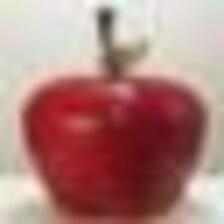
\includegraphics[width=.7\linewidth]{figures/CIFAR100/example_1.jpg}
        \captionsetup{labelformat=empty, justification=centering, font=scriptsize}
        \caption{\emph{Apple}}
      \end{figure}
    \end{column}
    \begin{column}{0.2\textwidth}
      \begin{figure}
        \centering
        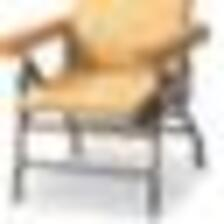
\includegraphics[width=.7\linewidth]{figures/CIFAR100/example_2.jpg}
        \captionsetup{labelformat=empty, justification=centering, font=scriptsize}
        \caption{\emph{Chair}}
      \end{figure}
    \end{column}
    \begin{column}{0.2\textwidth}
      \begin{figure}
        \centering
        
\includegraphics[width=.7\linewidth]{figures/CIFAR100/example_3.jpg}
        \captionsetup{labelformat=empty, justification=centering, font=scriptsize}
        \caption{\emph{Lobster}}
      \end{figure}
    \end{column}
  \end{columns}

  \rule{\linewidth}{0.4pt}

  \begin{columns}
    \begin{column}{0.35\textwidth}
      \alert{{\large iNaturalist19}}
      \begin{itemize}
        \item 1010 classes
        \item 8 hierarchy levels
      \end{itemize}
    \end{column}
    \begin{column}{0.2\textwidth}
      \begin{figure}
        \centering
        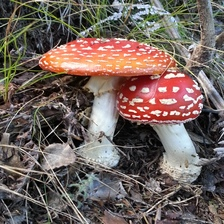
\includegraphics[width=.7\linewidth]{figures/iNaturalist19/example_1.jpg}
        \captionsetup{labelformat=empty, justification=centering, font=scriptsize}
        \caption{\emph{Amanita Muscaria}}
      \end{figure}
    \end{column}
    \begin{column}{0.2\textwidth}
      \begin{figure}
        \centering
        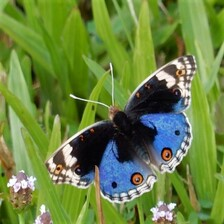
\includegraphics[width=.7\linewidth]{figures/iNaturalist19/example_2.jpg}
        \captionsetup{labelformat=empty, justification=centering, font=scriptsize}
        \caption{\emph{Junonia Orithya}}
      \end{figure}
    \end{column}
    \begin{column}{0.2\textwidth}
      \begin{figure}
        \centering
        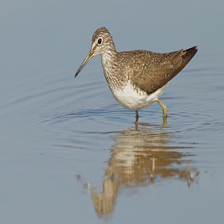
\includegraphics[width=.7\linewidth]{figures/iNaturalist19/example_3.jpg}
        \captionsetup{labelformat=empty, justification=centering, font=scriptsize}
        \caption{\emph{Tringa Ochropus}}
      \end{figure}
    \end{column}
  \end{columns}

  \rule{\linewidth}{0.4pt}

  \begin{columns}
    \begin{column}{0.35\textwidth}
      \alert{{\large tieredImageNet}}
      \begin{itemize}
        \item 608 classes
        \item 13 hierarchy levels
      \end{itemize}
    \end{column}
    \begin{column}{0.2\textwidth}
      \begin{figure}
        \centering
        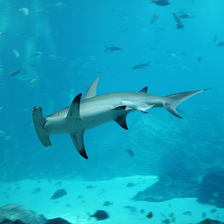
\includegraphics[width=.7\linewidth]{figures/tieredImageNet/example_1.jpg}
        \captionsetup{labelformat=empty, justification=centering, font=scriptsize}
        \caption{\emph{Hammerhead}}
      \end{figure}
    \end{column}
    \begin{column}{0.2\textwidth}
      \begin{figure}
        \centering
        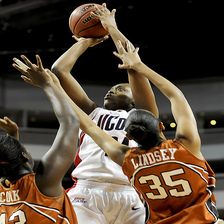
\includegraphics[width=.7\linewidth]{figures/tieredImageNet/example_2.jpg}
        \captionsetup{labelformat=empty, justification=centering, font=scriptsize}
        \caption{\emph{Basketball}}
      \end{figure}
    \end{column}
    \begin{column}{0.2\textwidth}
      \begin{figure}
        \centering
        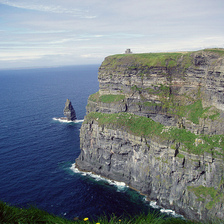
\includegraphics[width=.7\linewidth]{figures/tieredImageNet/example_3.jpg}
        \captionsetup{labelformat=empty, justification=centering, font=scriptsize}
        \caption{\emph{Cliff}}
      \end{figure}
    \end{column}
  \end{columns}

  \note[item]{I datasets utilizzati negli esperimenti sono CIFAR-100,
    iNaturalist19, tieredImageNet.}
  \note[item]{CIFAR-100 è un dataset di immagini a bassa risoluzione, 100
    classi per le quali è definita una gerarchia a 6 livelli.}
  \note[item]{iNaturaluralist sono foto di soggetti nautarali e le etichette
    associate sono il nome scientifico. 1010 classi e gerarchia a 8 livelli}
  \note[item]{tieredImageNet è un sotto insieme di ImageNet, 608 classi e 13
    livelli di gerarchia.}
\end{frame}


\begin{frame}{Experiments | Metrics}
  Let $\bm{M}$ be the \alert{confusion matrix} \\
  and $\bm{D}$ the \alert{distances matrix} previously introduced.
  \vspace{0.5cm}
  \begin{spreadlines}{15pt}
  \begin{align*}
    \text{Error Rate} &:=
      \frac{\sum \bm{M} - \text{tr} \, \bm{M}}{\sum \bm{M}} \\
    \text{Hierarchical Distance} &:=
      \frac{\sum \bm{M} \odot \bm{D}}{\sum \bm{M}} \\
    \text{Hierarchical Distance Mistake} &:=
      \frac{\sum \bm{M} \odot \bm{D}}{\sum \bm{M} - \text{tr} \, \bm{M}}
  \end{align*}
  \end{spreadlines}

  \note[Item]{Per misurare le performance del modello abbiamo fatto riscorso a
  3 metriche: Error Rate, Hiearchical Distance e Hiearchical Distance Mistake.}
  \note[item]{Queste possono essere definite a partire dalla matrice di
  confusione M e dalla matrice delle distaze D (tipo quella precedentemente
  introdotta).}
  \note[item]{L'Error Rate Il numero di errori commessi diviso il numero di
  esempi nel dataset di Test.}
  \note[item]{Hierarchical Distace la si ottiene moltiplicando M con D elemento
  per elemento, sommando le entrate della matrice risultante e dividendo per il
  totale degli esempi.}
  \note[item]{In Hierarchical distance Mistake nel denominatore è il numero di errori.}
  \note[item]{Error Rate è un indicatore di quanti errori il modello commette,
  mentre Hieararchical Distance Mistake quantifica la gravità di tali errori
  utilizzando come pesi le distanze nella gerarchia.}
\end{frame}


\begin{frame}{Experiments | Results}
  %% Creator: Matplotlib, PGF backend
%%
%% To include the figure in your LaTeX document, write
%%   \input{<filename>.pgf}
%%
%% Make sure the required packages are loaded in your preamble
%%   \usepackage{pgf}
%%
%% Also ensure that all the required font packages are loaded; for instance,
%% the lmodern package is sometimes necessary when using math font.
%%   \usepackage{lmodern}
%%
%% Figures using additional raster images can only be included by \input if
%% they are in the same directory as the main LaTeX file. For loading figures
%% from other directories you can use the `import` package
%%   \usepackage{import}
%%
%% and then include the figures with
%%   \import{<path to file>}{<filename>.pgf}
%%
%% Matplotlib used the following preamble
%%   
%%   \usepackage{fontspec}
%%   \setmainfont{DejaVuSerif.ttf}[Path=\detokenize{/Users/simo/.local/share/virtualenvs/master-thesis-code/lib/python3.10/site-packages/matplotlib/mpl-data/fonts/ttf/}]
%%   \setsansfont{DejaVuSans.ttf}[Path=\detokenize{/Users/simo/.local/share/virtualenvs/master-thesis-code/lib/python3.10/site-packages/matplotlib/mpl-data/fonts/ttf/}]
%%   \setmonofont{DejaVuSansMono.ttf}[Path=\detokenize{/Users/simo/.local/share/virtualenvs/master-thesis-code/lib/python3.10/site-packages/matplotlib/mpl-data/fonts/ttf/}]
%%   \makeatletter\@ifpackageloaded{underscore}{}{\usepackage[strings]{underscore}}\makeatother
%%
\begingroup%
\makeatletter%
\begin{pgfpicture}%
\pgfpathrectangle{\pgfpointorigin}{\pgfqpoint{4.251970in}{2.627862in}}%
\pgfusepath{use as bounding box, clip}%
\begin{pgfscope}%
\pgfsetbuttcap%
\pgfsetmiterjoin%
\definecolor{currentfill}{rgb}{0.980392,0.980392,0.980392}%
\pgfsetfillcolor{currentfill}%
\pgfsetlinewidth{0.000000pt}%
\definecolor{currentstroke}{rgb}{1.000000,1.000000,1.000000}%
\pgfsetstrokecolor{currentstroke}%
\pgfsetdash{}{0pt}%
\pgfpathmoveto{\pgfqpoint{0.000000in}{0.000000in}}%
\pgfpathlineto{\pgfqpoint{4.251970in}{0.000000in}}%
\pgfpathlineto{\pgfqpoint{4.251970in}{2.627862in}}%
\pgfpathlineto{\pgfqpoint{0.000000in}{2.627862in}}%
\pgfpathlineto{\pgfqpoint{0.000000in}{0.000000in}}%
\pgfpathclose%
\pgfusepath{fill}%
\end{pgfscope}%
\begin{pgfscope}%
\pgfsetbuttcap%
\pgfsetmiterjoin%
\definecolor{currentfill}{rgb}{0.917647,0.917647,0.949020}%
\pgfsetfillcolor{currentfill}%
\pgfsetlinewidth{0.000000pt}%
\definecolor{currentstroke}{rgb}{0.000000,0.000000,0.000000}%
\pgfsetstrokecolor{currentstroke}%
\pgfsetstrokeopacity{0.000000}%
\pgfsetdash{}{0pt}%
\pgfpathmoveto{\pgfqpoint{0.956688in}{0.387285in}}%
\pgfpathlineto{\pgfqpoint{2.790353in}{0.387285in}}%
\pgfpathlineto{\pgfqpoint{2.790353in}{2.390228in}}%
\pgfpathlineto{\pgfqpoint{0.956688in}{2.390228in}}%
\pgfpathlineto{\pgfqpoint{0.956688in}{0.387285in}}%
\pgfpathclose%
\pgfusepath{fill}%
\end{pgfscope}%
\begin{pgfscope}%
\definecolor{textcolor}{rgb}{0.137255,0.215686,0.231373}%
\pgfsetstrokecolor{textcolor}%
\pgfsetfillcolor{textcolor}%
\pgftext[x=1.160428in,y=0.248396in,,top]{\color{textcolor}\sffamily\fontsize{8.000000}{9.600000}\selectfont 27.0}%
\end{pgfscope}%
\begin{pgfscope}%
\definecolor{textcolor}{rgb}{0.137255,0.215686,0.231373}%
\pgfsetstrokecolor{textcolor}%
\pgfsetfillcolor{textcolor}%
\pgftext[x=1.466039in,y=0.248396in,,top]{\color{textcolor}\sffamily\fontsize{8.000000}{9.600000}\selectfont 27.3}%
\end{pgfscope}%
\begin{pgfscope}%
\definecolor{textcolor}{rgb}{0.137255,0.215686,0.231373}%
\pgfsetstrokecolor{textcolor}%
\pgfsetfillcolor{textcolor}%
\pgftext[x=1.771650in,y=0.248396in,,top]{\color{textcolor}\sffamily\fontsize{8.000000}{9.600000}\selectfont 27.6}%
\end{pgfscope}%
\begin{pgfscope}%
\definecolor{textcolor}{rgb}{0.137255,0.215686,0.231373}%
\pgfsetstrokecolor{textcolor}%
\pgfsetfillcolor{textcolor}%
\pgftext[x=2.077261in,y=0.248396in,,top]{\color{textcolor}\sffamily\fontsize{8.000000}{9.600000}\selectfont 27.9}%
\end{pgfscope}%
\begin{pgfscope}%
\definecolor{textcolor}{rgb}{0.137255,0.215686,0.231373}%
\pgfsetstrokecolor{textcolor}%
\pgfsetfillcolor{textcolor}%
\pgftext[x=2.382872in,y=0.248396in,,top]{\color{textcolor}\sffamily\fontsize{8.000000}{9.600000}\selectfont 28.2}%
\end{pgfscope}%
\begin{pgfscope}%
\definecolor{textcolor}{rgb}{0.137255,0.215686,0.231373}%
\pgfsetstrokecolor{textcolor}%
\pgfsetfillcolor{textcolor}%
\pgftext[x=2.790353in,y=0.248396in,,top]{\color{textcolor}\sffamily\fontsize{8.000000}{9.600000}\selectfont Error \%}%
\end{pgfscope}%
\begin{pgfscope}%
\definecolor{textcolor}{rgb}{0.137255,0.215686,0.231373}%
\pgfsetstrokecolor{textcolor}%
\pgfsetfillcolor{textcolor}%
\pgftext[x=0.570403in, y=0.499149in, left, base]{\color{textcolor}\sffamily\fontsize{8.000000}{9.600000}\selectfont 2.26}%
\end{pgfscope}%
\begin{pgfscope}%
\definecolor{textcolor}{rgb}{0.137255,0.215686,0.231373}%
\pgfsetstrokecolor{textcolor}%
\pgfsetfillcolor{textcolor}%
\pgftext[x=0.570403in, y=0.807294in, left, base]{\color{textcolor}\sffamily\fontsize{8.000000}{9.600000}\selectfont 2.30}%
\end{pgfscope}%
\begin{pgfscope}%
\definecolor{textcolor}{rgb}{0.137255,0.215686,0.231373}%
\pgfsetstrokecolor{textcolor}%
\pgfsetfillcolor{textcolor}%
\pgftext[x=0.570403in, y=1.115439in, left, base]{\color{textcolor}\sffamily\fontsize{8.000000}{9.600000}\selectfont 2.34}%
\end{pgfscope}%
\begin{pgfscope}%
\definecolor{textcolor}{rgb}{0.137255,0.215686,0.231373}%
\pgfsetstrokecolor{textcolor}%
\pgfsetfillcolor{textcolor}%
\pgftext[x=0.570403in, y=1.423583in, left, base]{\color{textcolor}\sffamily\fontsize{8.000000}{9.600000}\selectfont 2.38}%
\end{pgfscope}%
\begin{pgfscope}%
\definecolor{textcolor}{rgb}{0.137255,0.215686,0.231373}%
\pgfsetstrokecolor{textcolor}%
\pgfsetfillcolor{textcolor}%
\pgftext[x=0.570403in, y=1.731728in, left, base]{\color{textcolor}\sffamily\fontsize{8.000000}{9.600000}\selectfont 2.42}%
\end{pgfscope}%
\begin{pgfscope}%
\definecolor{textcolor}{rgb}{0.137255,0.215686,0.231373}%
\pgfsetstrokecolor{textcolor}%
\pgfsetfillcolor{textcolor}%
\pgftext[x=0.570403in, y=2.039873in, left, base]{\color{textcolor}\sffamily\fontsize{8.000000}{9.600000}\selectfont 2.46}%
\end{pgfscope}%
\begin{pgfscope}%
\definecolor{textcolor}{rgb}{0.137255,0.215686,0.231373}%
\pgfsetstrokecolor{textcolor}%
\pgfsetfillcolor{textcolor}%
\pgftext[x=0.155581in, y=2.401783in, left, base]{\color{textcolor}\sffamily\fontsize{8.000000}{9.600000}\selectfont Hierarchical}%
\end{pgfscope}%
\begin{pgfscope}%
\definecolor{textcolor}{rgb}{0.137255,0.215686,0.231373}%
\pgfsetstrokecolor{textcolor}%
\pgfsetfillcolor{textcolor}%
\pgftext[x=0.095142in, y=2.277370in, left, base]{\color{textcolor}\sffamily\fontsize{8.000000}{9.600000}\selectfont dist. mistake}%
\end{pgfscope}%
\begin{pgfscope}%
\pgfpathrectangle{\pgfqpoint{0.956688in}{0.387285in}}{\pgfqpoint{1.833666in}{2.002942in}}%
\pgfusepath{clip}%
\pgfsetbuttcap%
\pgfsetroundjoin%
\pgfsetlinewidth{0.752812pt}%
\definecolor{currentstroke}{rgb}{0.298039,0.447059,0.690196}%
\pgfsetstrokecolor{currentstroke}%
\pgfsetdash{}{0pt}%
\pgfpathmoveto{\pgfqpoint{1.807951in}{1.911346in}}%
\pgfpathlineto{\pgfqpoint{2.660332in}{1.911346in}}%
\pgfusepath{stroke}%
\end{pgfscope}%
\begin{pgfscope}%
\pgfpathrectangle{\pgfqpoint{0.956688in}{0.387285in}}{\pgfqpoint{1.833666in}{2.002942in}}%
\pgfusepath{clip}%
\pgfsetbuttcap%
\pgfsetroundjoin%
\pgfsetlinewidth{0.752812pt}%
\definecolor{currentstroke}{rgb}{0.298039,0.447059,0.690196}%
\pgfsetstrokecolor{currentstroke}%
\pgfsetdash{}{0pt}%
\pgfpathmoveto{\pgfqpoint{2.234141in}{1.789100in}}%
\pgfpathlineto{\pgfqpoint{2.234141in}{2.033592in}}%
\pgfusepath{stroke}%
\end{pgfscope}%
\begin{pgfscope}%
\pgfpathrectangle{\pgfqpoint{0.956688in}{0.387285in}}{\pgfqpoint{1.833666in}{2.002942in}}%
\pgfusepath{clip}%
\pgfsetbuttcap%
\pgfsetroundjoin%
\pgfsetlinewidth{0.752812pt}%
\definecolor{currentstroke}{rgb}{0.921569,0.505882,0.105882}%
\pgfsetstrokecolor{currentstroke}%
\pgfsetdash{}{0pt}%
\pgfpathmoveto{\pgfqpoint{1.609789in}{0.685162in}}%
\pgfpathlineto{\pgfqpoint{2.263571in}{0.685162in}}%
\pgfusepath{stroke}%
\end{pgfscope}%
\begin{pgfscope}%
\pgfpathrectangle{\pgfqpoint{0.956688in}{0.387285in}}{\pgfqpoint{1.833666in}{2.002942in}}%
\pgfusepath{clip}%
\pgfsetbuttcap%
\pgfsetroundjoin%
\pgfsetlinewidth{0.752812pt}%
\definecolor{currentstroke}{rgb}{0.921569,0.505882,0.105882}%
\pgfsetstrokecolor{currentstroke}%
\pgfsetdash{}{0pt}%
\pgfpathmoveto{\pgfqpoint{1.936680in}{0.605056in}}%
\pgfpathlineto{\pgfqpoint{1.936680in}{0.765268in}}%
\pgfusepath{stroke}%
\end{pgfscope}%
\begin{pgfscope}%
\pgfpathrectangle{\pgfqpoint{0.956688in}{0.387285in}}{\pgfqpoint{1.833666in}{2.002942in}}%
\pgfusepath{clip}%
\pgfsetbuttcap%
\pgfsetroundjoin%
\pgfsetlinewidth{0.752812pt}%
\definecolor{currentstroke}{rgb}{0.078431,0.690196,0.239216}%
\pgfsetstrokecolor{currentstroke}%
\pgfsetdash{}{0pt}%
\pgfpathmoveto{\pgfqpoint{1.283327in}{1.024880in}}%
\pgfpathlineto{\pgfqpoint{2.084756in}{1.024880in}}%
\pgfusepath{stroke}%
\end{pgfscope}%
\begin{pgfscope}%
\pgfpathrectangle{\pgfqpoint{0.956688in}{0.387285in}}{\pgfqpoint{1.833666in}{2.002942in}}%
\pgfusepath{clip}%
\pgfsetbuttcap%
\pgfsetroundjoin%
\pgfsetlinewidth{0.752812pt}%
\definecolor{currentstroke}{rgb}{0.078431,0.690196,0.239216}%
\pgfsetstrokecolor{currentstroke}%
\pgfsetdash{}{0pt}%
\pgfpathmoveto{\pgfqpoint{1.684042in}{0.841201in}}%
\pgfpathlineto{\pgfqpoint{1.684042in}{1.208559in}}%
\pgfusepath{stroke}%
\end{pgfscope}%
\begin{pgfscope}%
\pgfpathrectangle{\pgfqpoint{0.956688in}{0.387285in}}{\pgfqpoint{1.833666in}{2.002942in}}%
\pgfusepath{clip}%
\pgfsetbuttcap%
\pgfsetroundjoin%
\definecolor{currentfill}{rgb}{0.298039,0.447059,0.690196}%
\pgfsetfillcolor{currentfill}%
\pgfsetlinewidth{0.000000pt}%
\definecolor{currentstroke}{rgb}{0.298039,0.447059,0.690196}%
\pgfsetstrokecolor{currentstroke}%
\pgfsetdash{}{0pt}%
\pgfsys@defobject{currentmarker}{\pgfqpoint{-0.048611in}{-0.048611in}}{\pgfqpoint{0.048611in}{0.048611in}}{%
\pgfpathmoveto{\pgfqpoint{0.000000in}{-0.048611in}}%
\pgfpathcurveto{\pgfqpoint{0.012892in}{-0.048611in}}{\pgfqpoint{0.025257in}{-0.043489in}}{\pgfqpoint{0.034373in}{-0.034373in}}%
\pgfpathcurveto{\pgfqpoint{0.043489in}{-0.025257in}}{\pgfqpoint{0.048611in}{-0.012892in}}{\pgfqpoint{0.048611in}{0.000000in}}%
\pgfpathcurveto{\pgfqpoint{0.048611in}{0.012892in}}{\pgfqpoint{0.043489in}{0.025257in}}{\pgfqpoint{0.034373in}{0.034373in}}%
\pgfpathcurveto{\pgfqpoint{0.025257in}{0.043489in}}{\pgfqpoint{0.012892in}{0.048611in}}{\pgfqpoint{0.000000in}{0.048611in}}%
\pgfpathcurveto{\pgfqpoint{-0.012892in}{0.048611in}}{\pgfqpoint{-0.025257in}{0.043489in}}{\pgfqpoint{-0.034373in}{0.034373in}}%
\pgfpathcurveto{\pgfqpoint{-0.043489in}{0.025257in}}{\pgfqpoint{-0.048611in}{0.012892in}}{\pgfqpoint{-0.048611in}{0.000000in}}%
\pgfpathcurveto{\pgfqpoint{-0.048611in}{-0.012892in}}{\pgfqpoint{-0.043489in}{-0.025257in}}{\pgfqpoint{-0.034373in}{-0.034373in}}%
\pgfpathcurveto{\pgfqpoint{-0.025257in}{-0.043489in}}{\pgfqpoint{-0.012892in}{-0.048611in}}{\pgfqpoint{0.000000in}{-0.048611in}}%
\pgfpathlineto{\pgfqpoint{0.000000in}{-0.048611in}}%
\pgfpathclose%
\pgfusepath{fill}%
}%
\begin{pgfscope}%
\pgfsys@transformshift{2.234141in}{1.911346in}%
\pgfsys@useobject{currentmarker}{}%
\end{pgfscope}%
\end{pgfscope}%
\begin{pgfscope}%
\pgfpathrectangle{\pgfqpoint{0.956688in}{0.387285in}}{\pgfqpoint{1.833666in}{2.002942in}}%
\pgfusepath{clip}%
\pgfsetbuttcap%
\pgfsetroundjoin%
\definecolor{currentfill}{rgb}{0.921569,0.505882,0.105882}%
\pgfsetfillcolor{currentfill}%
\pgfsetlinewidth{0.000000pt}%
\definecolor{currentstroke}{rgb}{0.921569,0.505882,0.105882}%
\pgfsetstrokecolor{currentstroke}%
\pgfsetdash{}{0pt}%
\pgfsys@defobject{currentmarker}{\pgfqpoint{-0.048611in}{-0.048611in}}{\pgfqpoint{0.048611in}{0.048611in}}{%
\pgfpathmoveto{\pgfqpoint{0.000000in}{-0.048611in}}%
\pgfpathcurveto{\pgfqpoint{0.012892in}{-0.048611in}}{\pgfqpoint{0.025257in}{-0.043489in}}{\pgfqpoint{0.034373in}{-0.034373in}}%
\pgfpathcurveto{\pgfqpoint{0.043489in}{-0.025257in}}{\pgfqpoint{0.048611in}{-0.012892in}}{\pgfqpoint{0.048611in}{0.000000in}}%
\pgfpathcurveto{\pgfqpoint{0.048611in}{0.012892in}}{\pgfqpoint{0.043489in}{0.025257in}}{\pgfqpoint{0.034373in}{0.034373in}}%
\pgfpathcurveto{\pgfqpoint{0.025257in}{0.043489in}}{\pgfqpoint{0.012892in}{0.048611in}}{\pgfqpoint{0.000000in}{0.048611in}}%
\pgfpathcurveto{\pgfqpoint{-0.012892in}{0.048611in}}{\pgfqpoint{-0.025257in}{0.043489in}}{\pgfqpoint{-0.034373in}{0.034373in}}%
\pgfpathcurveto{\pgfqpoint{-0.043489in}{0.025257in}}{\pgfqpoint{-0.048611in}{0.012892in}}{\pgfqpoint{-0.048611in}{0.000000in}}%
\pgfpathcurveto{\pgfqpoint{-0.048611in}{-0.012892in}}{\pgfqpoint{-0.043489in}{-0.025257in}}{\pgfqpoint{-0.034373in}{-0.034373in}}%
\pgfpathcurveto{\pgfqpoint{-0.025257in}{-0.043489in}}{\pgfqpoint{-0.012892in}{-0.048611in}}{\pgfqpoint{0.000000in}{-0.048611in}}%
\pgfpathlineto{\pgfqpoint{0.000000in}{-0.048611in}}%
\pgfpathclose%
\pgfusepath{fill}%
}%
\begin{pgfscope}%
\pgfsys@transformshift{1.936680in}{0.685162in}%
\pgfsys@useobject{currentmarker}{}%
\end{pgfscope}%
\end{pgfscope}%
\begin{pgfscope}%
\pgfpathrectangle{\pgfqpoint{0.956688in}{0.387285in}}{\pgfqpoint{1.833666in}{2.002942in}}%
\pgfusepath{clip}%
\pgfsetbuttcap%
\pgfsetroundjoin%
\definecolor{currentfill}{rgb}{0.078431,0.690196,0.239216}%
\pgfsetfillcolor{currentfill}%
\pgfsetlinewidth{0.000000pt}%
\definecolor{currentstroke}{rgb}{0.078431,0.690196,0.239216}%
\pgfsetstrokecolor{currentstroke}%
\pgfsetdash{}{0pt}%
\pgfsys@defobject{currentmarker}{\pgfqpoint{-0.048611in}{-0.048611in}}{\pgfqpoint{0.048611in}{0.048611in}}{%
\pgfpathmoveto{\pgfqpoint{0.000000in}{-0.048611in}}%
\pgfpathcurveto{\pgfqpoint{0.012892in}{-0.048611in}}{\pgfqpoint{0.025257in}{-0.043489in}}{\pgfqpoint{0.034373in}{-0.034373in}}%
\pgfpathcurveto{\pgfqpoint{0.043489in}{-0.025257in}}{\pgfqpoint{0.048611in}{-0.012892in}}{\pgfqpoint{0.048611in}{0.000000in}}%
\pgfpathcurveto{\pgfqpoint{0.048611in}{0.012892in}}{\pgfqpoint{0.043489in}{0.025257in}}{\pgfqpoint{0.034373in}{0.034373in}}%
\pgfpathcurveto{\pgfqpoint{0.025257in}{0.043489in}}{\pgfqpoint{0.012892in}{0.048611in}}{\pgfqpoint{0.000000in}{0.048611in}}%
\pgfpathcurveto{\pgfqpoint{-0.012892in}{0.048611in}}{\pgfqpoint{-0.025257in}{0.043489in}}{\pgfqpoint{-0.034373in}{0.034373in}}%
\pgfpathcurveto{\pgfqpoint{-0.043489in}{0.025257in}}{\pgfqpoint{-0.048611in}{0.012892in}}{\pgfqpoint{-0.048611in}{0.000000in}}%
\pgfpathcurveto{\pgfqpoint{-0.048611in}{-0.012892in}}{\pgfqpoint{-0.043489in}{-0.025257in}}{\pgfqpoint{-0.034373in}{-0.034373in}}%
\pgfpathcurveto{\pgfqpoint{-0.025257in}{-0.043489in}}{\pgfqpoint{-0.012892in}{-0.048611in}}{\pgfqpoint{0.000000in}{-0.048611in}}%
\pgfpathlineto{\pgfqpoint{0.000000in}{-0.048611in}}%
\pgfpathclose%
\pgfusepath{fill}%
}%
\begin{pgfscope}%
\pgfsys@transformshift{1.684042in}{1.024880in}%
\pgfsys@useobject{currentmarker}{}%
\end{pgfscope}%
\end{pgfscope}%
\begin{pgfscope}%
\pgfsetrectcap%
\pgfsetmiterjoin%
\pgfsetlinewidth{1.003750pt}%
\definecolor{currentstroke}{rgb}{0.917647,0.917647,0.949020}%
\pgfsetstrokecolor{currentstroke}%
\pgfsetdash{}{0pt}%
\pgfpathmoveto{\pgfqpoint{0.956688in}{0.387285in}}%
\pgfpathlineto{\pgfqpoint{0.956688in}{2.390228in}}%
\pgfusepath{stroke}%
\end{pgfscope}%
\begin{pgfscope}%
\pgfsetrectcap%
\pgfsetmiterjoin%
\pgfsetlinewidth{1.003750pt}%
\definecolor{currentstroke}{rgb}{0.917647,0.917647,0.949020}%
\pgfsetstrokecolor{currentstroke}%
\pgfsetdash{}{0pt}%
\pgfpathmoveto{\pgfqpoint{2.790353in}{0.387285in}}%
\pgfpathlineto{\pgfqpoint{2.790353in}{2.390228in}}%
\pgfusepath{stroke}%
\end{pgfscope}%
\begin{pgfscope}%
\pgfsetrectcap%
\pgfsetmiterjoin%
\pgfsetlinewidth{1.003750pt}%
\definecolor{currentstroke}{rgb}{0.917647,0.917647,0.949020}%
\pgfsetstrokecolor{currentstroke}%
\pgfsetdash{}{0pt}%
\pgfpathmoveto{\pgfqpoint{0.956688in}{0.387285in}}%
\pgfpathlineto{\pgfqpoint{2.790353in}{0.387285in}}%
\pgfusepath{stroke}%
\end{pgfscope}%
\begin{pgfscope}%
\pgfsetrectcap%
\pgfsetmiterjoin%
\pgfsetlinewidth{1.003750pt}%
\definecolor{currentstroke}{rgb}{0.917647,0.917647,0.949020}%
\pgfsetstrokecolor{currentstroke}%
\pgfsetdash{}{0pt}%
\pgfpathmoveto{\pgfqpoint{0.956688in}{2.390228in}}%
\pgfpathlineto{\pgfqpoint{2.790353in}{2.390228in}}%
\pgfusepath{stroke}%
\end{pgfscope}%
\begin{pgfscope}%
\pgfsetbuttcap%
\pgfsetroundjoin%
\definecolor{currentfill}{rgb}{0.298039,0.447059,0.690196}%
\pgfsetfillcolor{currentfill}%
\pgfsetlinewidth{0.000000pt}%
\definecolor{currentstroke}{rgb}{0.298039,0.447059,0.690196}%
\pgfsetstrokecolor{currentstroke}%
\pgfsetdash{}{0pt}%
\pgfsys@defobject{currentmarker}{\pgfqpoint{-0.048611in}{-0.048611in}}{\pgfqpoint{0.048611in}{0.048611in}}{%
\pgfpathmoveto{\pgfqpoint{0.000000in}{-0.048611in}}%
\pgfpathcurveto{\pgfqpoint{0.012892in}{-0.048611in}}{\pgfqpoint{0.025257in}{-0.043489in}}{\pgfqpoint{0.034373in}{-0.034373in}}%
\pgfpathcurveto{\pgfqpoint{0.043489in}{-0.025257in}}{\pgfqpoint{0.048611in}{-0.012892in}}{\pgfqpoint{0.048611in}{0.000000in}}%
\pgfpathcurveto{\pgfqpoint{0.048611in}{0.012892in}}{\pgfqpoint{0.043489in}{0.025257in}}{\pgfqpoint{0.034373in}{0.034373in}}%
\pgfpathcurveto{\pgfqpoint{0.025257in}{0.043489in}}{\pgfqpoint{0.012892in}{0.048611in}}{\pgfqpoint{0.000000in}{0.048611in}}%
\pgfpathcurveto{\pgfqpoint{-0.012892in}{0.048611in}}{\pgfqpoint{-0.025257in}{0.043489in}}{\pgfqpoint{-0.034373in}{0.034373in}}%
\pgfpathcurveto{\pgfqpoint{-0.043489in}{0.025257in}}{\pgfqpoint{-0.048611in}{0.012892in}}{\pgfqpoint{-0.048611in}{0.000000in}}%
\pgfpathcurveto{\pgfqpoint{-0.048611in}{-0.012892in}}{\pgfqpoint{-0.043489in}{-0.025257in}}{\pgfqpoint{-0.034373in}{-0.034373in}}%
\pgfpathcurveto{\pgfqpoint{-0.025257in}{-0.043489in}}{\pgfqpoint{-0.012892in}{-0.048611in}}{\pgfqpoint{0.000000in}{-0.048611in}}%
\pgfpathlineto{\pgfqpoint{0.000000in}{-0.048611in}}%
\pgfpathclose%
\pgfusepath{fill}%
}%
\begin{pgfscope}%
\pgfsys@transformshift{3.001464in}{1.784047in}%
\pgfsys@useobject{currentmarker}{}%
\end{pgfscope}%
\end{pgfscope}%
\begin{pgfscope}%
\definecolor{textcolor}{rgb}{0.137255,0.215686,0.231373}%
\pgfsetstrokecolor{textcolor}%
\pgfsetfillcolor{textcolor}%
\pgftext[x=3.201464in, y=1.818921in, left, base]{\color{textcolor}\sffamily\fontsize{8.000000}{9.600000}\selectfont One-hot enc.}%
\end{pgfscope}%
\begin{pgfscope}%
\definecolor{textcolor}{rgb}{0.137255,0.215686,0.231373}%
\pgfsetstrokecolor{textcolor}%
\pgfsetfillcolor{textcolor}%
\pgftext[x=3.201464in, y=1.694507in, left, base]{\color{textcolor}\sffamily\fontsize{8.000000}{9.600000}\selectfont Cross Entropy}%
\end{pgfscope}%
\begin{pgfscope}%
\pgfsetbuttcap%
\pgfsetroundjoin%
\definecolor{currentfill}{rgb}{0.921569,0.505882,0.105882}%
\pgfsetfillcolor{currentfill}%
\pgfsetlinewidth{0.000000pt}%
\definecolor{currentstroke}{rgb}{0.921569,0.505882,0.105882}%
\pgfsetstrokecolor{currentstroke}%
\pgfsetdash{}{0pt}%
\pgfsys@defobject{currentmarker}{\pgfqpoint{-0.048611in}{-0.048611in}}{\pgfqpoint{0.048611in}{0.048611in}}{%
\pgfpathmoveto{\pgfqpoint{0.000000in}{-0.048611in}}%
\pgfpathcurveto{\pgfqpoint{0.012892in}{-0.048611in}}{\pgfqpoint{0.025257in}{-0.043489in}}{\pgfqpoint{0.034373in}{-0.034373in}}%
\pgfpathcurveto{\pgfqpoint{0.043489in}{-0.025257in}}{\pgfqpoint{0.048611in}{-0.012892in}}{\pgfqpoint{0.048611in}{0.000000in}}%
\pgfpathcurveto{\pgfqpoint{0.048611in}{0.012892in}}{\pgfqpoint{0.043489in}{0.025257in}}{\pgfqpoint{0.034373in}{0.034373in}}%
\pgfpathcurveto{\pgfqpoint{0.025257in}{0.043489in}}{\pgfqpoint{0.012892in}{0.048611in}}{\pgfqpoint{0.000000in}{0.048611in}}%
\pgfpathcurveto{\pgfqpoint{-0.012892in}{0.048611in}}{\pgfqpoint{-0.025257in}{0.043489in}}{\pgfqpoint{-0.034373in}{0.034373in}}%
\pgfpathcurveto{\pgfqpoint{-0.043489in}{0.025257in}}{\pgfqpoint{-0.048611in}{0.012892in}}{\pgfqpoint{-0.048611in}{0.000000in}}%
\pgfpathcurveto{\pgfqpoint{-0.048611in}{-0.012892in}}{\pgfqpoint{-0.043489in}{-0.025257in}}{\pgfqpoint{-0.034373in}{-0.034373in}}%
\pgfpathcurveto{\pgfqpoint{-0.025257in}{-0.043489in}}{\pgfqpoint{-0.012892in}{-0.048611in}}{\pgfqpoint{0.000000in}{-0.048611in}}%
\pgfpathlineto{\pgfqpoint{0.000000in}{-0.048611in}}%
\pgfpathclose%
\pgfusepath{fill}%
}%
\begin{pgfscope}%
\pgfsys@transformshift{3.001464in}{1.385436in}%
\pgfsys@useobject{currentmarker}{}%
\end{pgfscope}%
\end{pgfscope}%
\begin{pgfscope}%
\definecolor{textcolor}{rgb}{0.137255,0.215686,0.231373}%
\pgfsetstrokecolor{textcolor}%
\pgfsetfillcolor{textcolor}%
\pgftext[x=3.201464in, y=1.420310in, left, base]{\color{textcolor}\sffamily\fontsize{8.000000}{9.600000}\selectfont Hierarchical enc.}%
\end{pgfscope}%
\begin{pgfscope}%
\definecolor{textcolor}{rgb}{0.137255,0.215686,0.231373}%
\pgfsetstrokecolor{textcolor}%
\pgfsetfillcolor{textcolor}%
\pgftext[x=3.201464in, y=1.295896in, left, base]{\color{textcolor}\sffamily\fontsize{8.000000}{9.600000}\selectfont Cross Entropy}%
\end{pgfscope}%
\begin{pgfscope}%
\pgfsetbuttcap%
\pgfsetroundjoin%
\definecolor{currentfill}{rgb}{0.078431,0.690196,0.239216}%
\pgfsetfillcolor{currentfill}%
\pgfsetlinewidth{0.000000pt}%
\definecolor{currentstroke}{rgb}{0.078431,0.690196,0.239216}%
\pgfsetstrokecolor{currentstroke}%
\pgfsetdash{}{0pt}%
\pgfsys@defobject{currentmarker}{\pgfqpoint{-0.048611in}{-0.048611in}}{\pgfqpoint{0.048611in}{0.048611in}}{%
\pgfpathmoveto{\pgfqpoint{0.000000in}{-0.048611in}}%
\pgfpathcurveto{\pgfqpoint{0.012892in}{-0.048611in}}{\pgfqpoint{0.025257in}{-0.043489in}}{\pgfqpoint{0.034373in}{-0.034373in}}%
\pgfpathcurveto{\pgfqpoint{0.043489in}{-0.025257in}}{\pgfqpoint{0.048611in}{-0.012892in}}{\pgfqpoint{0.048611in}{0.000000in}}%
\pgfpathcurveto{\pgfqpoint{0.048611in}{0.012892in}}{\pgfqpoint{0.043489in}{0.025257in}}{\pgfqpoint{0.034373in}{0.034373in}}%
\pgfpathcurveto{\pgfqpoint{0.025257in}{0.043489in}}{\pgfqpoint{0.012892in}{0.048611in}}{\pgfqpoint{0.000000in}{0.048611in}}%
\pgfpathcurveto{\pgfqpoint{-0.012892in}{0.048611in}}{\pgfqpoint{-0.025257in}{0.043489in}}{\pgfqpoint{-0.034373in}{0.034373in}}%
\pgfpathcurveto{\pgfqpoint{-0.043489in}{0.025257in}}{\pgfqpoint{-0.048611in}{0.012892in}}{\pgfqpoint{-0.048611in}{0.000000in}}%
\pgfpathcurveto{\pgfqpoint{-0.048611in}{-0.012892in}}{\pgfqpoint{-0.043489in}{-0.025257in}}{\pgfqpoint{-0.034373in}{-0.034373in}}%
\pgfpathcurveto{\pgfqpoint{-0.025257in}{-0.043489in}}{\pgfqpoint{-0.012892in}{-0.048611in}}{\pgfqpoint{0.000000in}{-0.048611in}}%
\pgfpathlineto{\pgfqpoint{0.000000in}{-0.048611in}}%
\pgfpathclose%
\pgfusepath{fill}%
}%
\begin{pgfscope}%
\pgfsys@transformshift{3.001464in}{0.986825in}%
\pgfsys@useobject{currentmarker}{}%
\end{pgfscope}%
\end{pgfscope}%
\begin{pgfscope}%
\definecolor{textcolor}{rgb}{0.137255,0.215686,0.231373}%
\pgfsetstrokecolor{textcolor}%
\pgfsetfillcolor{textcolor}%
\pgftext[x=3.201464in, y=1.021699in, left, base]{\color{textcolor}\sffamily\fontsize{8.000000}{9.600000}\selectfont Description enc.}%
\end{pgfscope}%
\begin{pgfscope}%
\definecolor{textcolor}{rgb}{0.137255,0.215686,0.231373}%
\pgfsetstrokecolor{textcolor}%
\pgfsetfillcolor{textcolor}%
\pgftext[x=3.201464in, y=0.897285in, left, base]{\color{textcolor}\sffamily\fontsize{8.000000}{9.600000}\selectfont Cosine Distance}%
\end{pgfscope}%
\end{pgfpicture}%
\makeatother%
\endgroup%

  \note[item]{TODO}
\end{frame}
